\documentclass{article}

\usepackage[french]{babel}
\usepackage[utf8]{inputenc}
\usepackage[T1]{fontenc}
\usepackage{verbatim}
\usepackage{graphicx}
\usepackage{calc}
\usepackage{color}
\usepackage{float}

\title{Projet système \\ Mise en place d'une bibliothèque de threads}
\author{Gardon Henri, Ludovic Hofer, Pierre-Alain Pocquet, Tony
  Sanchez}

\begin{document}

	\maketitle
	\newpage
	\tableofcontents
	\newpage

	\section{Introduction}
	
	Au sein de ce projet nous nous attacherons à mettre en place une
    bibliothèque de gestion de threads. Cette dernière proposera une
    interface de programmation semblable à celle de pthread, à la
    différence près qu'un seul thread noyau sera utilisé.

	\section{Structures de données}

		\subsection{Représentation d'un thread}
		Au sein de notre bibliothèque de thread, nous avons choisi de les
		représenter en utilisant la structure suivante : \\
		\begin{verbatim}
		struct thread{
    ucontext_t context;
    /* Stack_id is used in order to work properly with valgrind */
    int stack_id;
    /* Status is needed in order to allow join to work properly */
    int status;
    struct thread * next;
    bool freeNeeded;
    /* retval is used in join and allow to store the return value */
    void * retval;
};
	\end{verbatim}
		Les différents champs de la structure ont les utilités 
		suivantes :
		\begin{itemize}
			\item \verb!context! :
			\item \verb!stack_id! :
			\item \verb!status! :
			\item \verb!next! : %TODO attribut toujours utile
			
		\end{itemize}		
		

		\subsection{Représentation des threads}
		Pour pouvoir gérer un ensemble de thread il a fallu que nous
        mettions en place une structure permettant d'en contenir un
        certain nombre, qui sera manipulée par les primitives internes
        à la bibliothèque que nous nous attacherons à présenter dans
        la suite de ce rapport.

			\subsubsection{Première version et utilisation d'un tableau}
			Dans en premier temps nous avons choisi d'utiliser un
            tableau pour représenter notre l'ensemble de thread que
            nous devions exécuter.  Si cette solution présente
            l'avantage d'être rapide à mettre au point et de pouvoir
            aboutir à un résultat fonctionnel, elle présente néanmoins
            certains inconvénients.
			
			Elle doit se limiter à un nombre de thread fixé par la
            bibliothèque, l'utilisateur peut donc potentiellement (et
            par exemple dans les cas de fonctions récursives se
            retrouver dans le cas où il dépasse cette limite.
			
			Cependant grâce à cette implementation nous avons tester
            très rapidement les problèmes d'algorithmique liés à la
            bibliothèque en se focalisant sur les fonctionnalités et
            non pas sur les spécificités d'implémentation.

			\subsubsection{Amélioration et passage listes}
			Après avoir réussi à mettre au point une version primaire
            mais fonctionnel de notre bibliothèque, nous avons décider
            de la faire évoluer en changeant la représentations
            interne de l'ensemble de threads gérés.  L'avantage de
            cette version été qu'elle nous permettait de gérer un
            nombre de thread non plus limité en interne, mais par les
            limites physique de l'ordinateur sur lequel elle
            s'exécutait.
			
			Dans un but de simplicité nous avions choisi d'utiliser
            des GLists au sein de cette version. Bien que nous
            éloignant des soucis de mise au point d'une telle
            structure et nous permettant une mise au point rapide,
            l'utilisation d'une API externe implique quelques
            problèmes que nous n'avions pas pris en compte.
			
			En effet la gestion de la mémoire s'est révélé plus
            complexe que ce que nous pensions, et notre bibliothèque
            laissée une empreinte mémoire après exécution.
            Rétrospectivement il aurait été plus intéressant
            d'utiliser une file pour gérer les différents threads. Ce
            dernier point sera abordé dans les améliorations possibles
            à la fin de ce rapport.
			

	\section{Fonctionnement de la bibliothèque}
	Nous nous attacherons dans cette partie à expliquer le
    fonctionnement interne de notre bibliothèque, et en particulier
     de la version gérant les threads sous forme de
    liste.

		\subsection{Ajout d'un thread}
		L'ajout d'un thread est fait par l'utilisateur en faisant 
		appel à la fonction \verb!thread_create()!
		

		\subsection{Recherche du prochain thread à exécuter}

		\subsection{Spécificités d'implémentation}
		
			\subsubsection{gestion des threads retournants des valeurs}
			description du wrapper
			
			\subsubsection{terminaison et libération de ressources}
			ici parler des fonctions end thread handling etc...
		

	\section{ordonnancement}
	Cette partie sera consacrée à expliquer plus finement comment
    l'ordonnacement des threads sera mise en place.

		\subsection{Sans ordonnanceur}
		l'ordonnancement au sein des différentes méthodes à la manière
        de pthread.

		\subsection{Version multi-coeur et changements}
		Parmi les objectifs à remplir, il nous avait été proposé de prendre
        en charge les architectures multi-coeurs en utilisant plusieurs
        threads noyaux. Deux possibilités nous avaient été proposées :
        \begin{itemize}
          \item Utiliser la fonction \verb!clone!
          \item Utiliser \verb!pthread! pour créer les threads noyaux.
        \end{itemize}
        Un collègue nous ayant hautement déconseillé d'utiliser la fonction
        \verb!clone! en raison des problèmes engendrés lorsque des fonctions
        de la librairie standard \verb!c! sont utilisées, nous avons préféré
        nous baser sur la librairie \verb!pthread!.
        \paragraph{}
        Afin de faire fonctionner ces threads noyaux, il était inévitable
        d'utiliser des mutex\footnote{Entre autre pour éviter que deux
          threads noyaux sélectionnent le même thread utilisateur.}, nous
        avons donc utilisés ceux de la librairie \verb!pthread!. 
        \paragraph{}
        Afin de faciliter le passage au multi-coeur, nous avons choisi
        de revenir aux threads noyaux entre deux exécutions de threads, ce
        qui permettait plus facilement de récupérer le prochain thread. Notre
        implémentation du pool de thread sous forme de liste a compliqué les
        choses pour ce passage étant donné que lorsqu'un élément est retiré
        de la liste de thread (après un \verb!thread_join!), il faut mettre
        à jour tous les éléments dont l'indice était supérieur à celui de
        l'élément retiré.
        \paragraph{}
        Afin de pouvoir essayer différents nombre de threads noyaux, nous
        avons défini une macro dans \verb!thread.c! définissant le nombre
        de ces threads. Il est d'ailleurs à noter que lorsque moins de
        threads utilisateurs sont actifs que de threads noyaux, nous
        n'évitons pas le fait d'avoir de l'attente active\footnote{Nous avons
          placé un \verb!sleep! sur un temps court afin de ne pas consommer
          trop de CPU à ne rien faire tout en évitant d'avoir un temps de
          réaction trop élevé.}.
        \paragraph{}
        Il est aussi à noter qu'avec le déploiement de cette fonctionnalité,
        nous avons eu de nouveaux bugs que nous n'avons pas tous réussi à
        éliminer, cependant ceux-ci ne se produisant que rarement et de façon
        aléatoire, nous n'avons pas réussi à les résoudre dans le temps
        imparti.

	\section{Tests et performance}
    Afin de pouvoir valider l'évolution du code, nous avons mis en place un
    système de validation se basant principalement sur le code fourni.
    Celui-ci permettait initialement de valider non seulement la bonne
    exécution des programmes, mais aussi l'absence de problèmes signalés par
    \verb!valgrind!. Cependant, à cause des problèmes de fuite mémoire lors
    de l'utilisation des {\em GList}, cette partie du test est rapidement
    devenue inutiles, tous les programmes de test échouant.
    \begin{figure}[H]
      \caption{Exemple d'exécution du module de test}
      \centering
      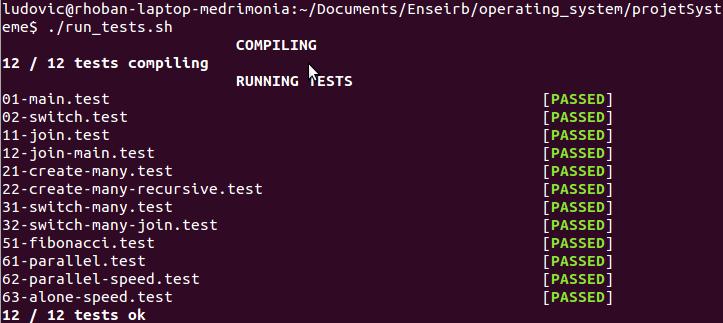
\includegraphics [width=\textwidth]{tests.png}
    \end{figure}
    \paragraph{}
    Ces tests nous ont permis de nous rendre compte de bugs dans des tests
    où nous ne les attendions pas lors de certaines modifications et leur
    diversité a aussi permis de couvrir des situations auxquels nous
    n'aurions pas forcément pensé.
    \paragraph{}
    Au niveau des performances, nous sommes conscients qu'il y a de
    nombreux problèmes qui nuisent à la performance, entre autre le fait que
    nous ayons une seule liste pour les threads, quelque soit leur statut. Il
    est facile d'imaginer une situation ou de très nombreux threads sont dans
    un statut \verb!TERMINATED!, attendant que quelqu'un vienne récupérer
    la valeur de retour, dans ce cas, \verb!next_thread! peut très bien
    demander de faire un nombre de tour de boucle dépendant du nombre de
    threads alors que si ces listes étaient distinguées, l'accès serait en
    temps constant.
    \paragraph{}
    Afin de comparer les performances de notre implémentation avec celle de
    pthread lors de l'utilisation de plusieurs coeurs, nous avons lancé
    exactement le même programme\footnote{Une simple boucle incrémentant une
      valeur} dans trois configurations différentes.
    \begin{itemize}
      \item Sans aucun thread, en séquentiel pur
      \item En utilisant uniquement pthread
      \item En utilisant notre implémentation de thread
    \end{itemize}
    \paragraph{}
    Dans les deux derniers cas, le nombre de thread était variable. Ce test
    s'est effectué sur {\em trelawney}\footnote{Une machine du {\em CREMI}}
    qui apparemment possède en tout cas 8 coeurs. Comme les temps
    d'exécutions variaient légèrement, le même procédé a été appliqué dans
    les deux cas, sur 5 exécutions, le temps minimal était conservé.
    \begin{figure}[H]
      \caption{Mesure de la performance en multi-coeur}
      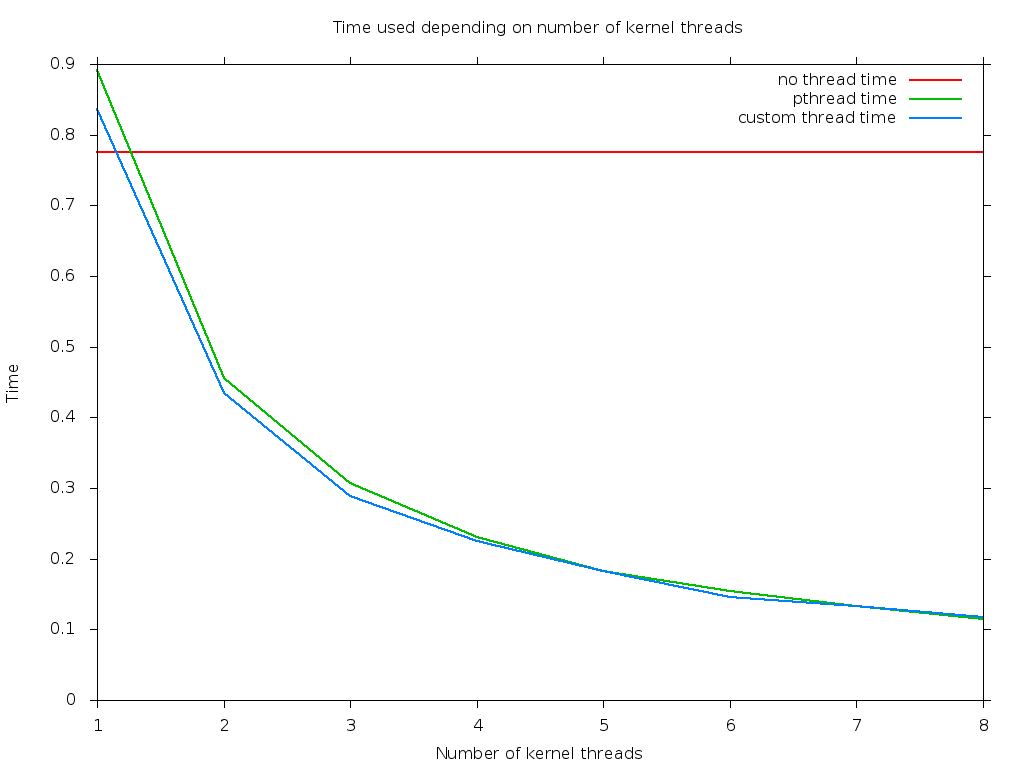
\includegraphics[width=\textwidth]{compare.png}
    \end{figure}
    \paragraph{}
    Nous avons pu vérifier que nous obtenions bien un gain de performance
    avec les threads noyaux, ce qui est normal étant donné que dans notre
    cas, nous nous sommes appuyé sur pthread pour créer les threads noyaux et
    que les threads utilisateurs n'ont donc pas de raison de redonner la main
    à des threads noyaux.
    % TODO éventuellement test comparant un grand nombre de thread sur le 
    % même coeur



	\section{Résultats}
    Si nous avons réussi à obtenir assez rapidement une première version
    fiable et fonctionnelle respectant les premiers tests en stockant les
    threads dans un tableau, le passage aux listes a déjà commencé à poser
    certains problèmes, car nous souhaitions éliminer toutes les fuites
    mémoires ce que nous n'avons pas réussi à résoudre, certains problèmes
    semblant venir de l'implémentation des GList elles mêmes.
    \paragraph
    Par la suite, les améliorations se sont révélées assez problématiques,
    puisque le seul objectif avancé que nous avons réussi à accomplir est le
    support des machines multi-processeurs et malgré le travail de débugage
    effectué, il reste parfois des problèmes que nous n'avons pas encore pu
    comprendre.

	\section{Perspectives}
    Tel qu'il est présenté, le projet pourrait difficilement être repris
    afin d'y ajouter d'autres fonctionnalités, idéalement, le code devrait
    être repris de zéro afin d'être plus clair. Il devrait être modularisé et
    bien plus commenté, avant tout au niveau du comportement des différentes
    fonctions.
    \paragraph{}
    Au niveau des performances, utiliser des files permettrait une insertion
    et un choix du prochain thread plus rapide. Une autre des priorités
    serait d'intégrer la préemption afin de ne plus se reposer sur un
    comportement coopératif. Il serait aussi intéressant que la bibliothèque
    dispose de ses propres mutex. Il faudrait aussi pouvoir permettre à des
    threads d'envoyer des signaux à d'autres, d'annuler d'autres threads ou
    encore de détecter les débordements de pile. Finalement, il serait
    intéressant de proposer des priorités aux threads ainsi que des moyens
    de choisir entre différentes politiques d'ordonnancement.

	\section{Conclusion}
    Ce projet nous a énormément appris sur les difficultés rencontrées lors
    de l'implémentation. Il nous a permis d'appliquer nos connaissance
    théoriques acquises lors des cours de programmation système et de système
    d'exploitation pour essayer de mettre en place une bibliothèque
    s'inspirant de celle dont nous avons pris l'habitude de nous servir.
    \paragraph{}
    Au vu de notre expérience, il nous paraît primordial d'avoir un module
    d'ordonnancement fournissant une interface claire afin de pouvoir
    implémenter les threads plus facilement. Effectivement, un grand nombre
    de nos problèmes de débugages provenaient du fait que les différents
    aspects n'étaient pas assez séparés et qu'il n'était pas clair de savoir
    quel comportement l'on attendait exactement d'une fonction. La gestion
    de la programmation multi-coeur aurait pu être grandement simplifiée si
    nous avions déjà disposé d'une fonction \verb!get_next_thread!
    permettant de récupérer le prochain thread sans avoir à se soucier des
    accès concurrents. La gestion de ceux-ci dans notre programme
    manquant encore de de clarté à la fin du projet.
    \paragraph{}
    Nous avons aussi pu constater que si une version minimaliste d'un
    gestionnaire de thread est relativement facile à implémenter, toutes les
    garanties qu'offre une librairie tel que {\em pthread} représentent un
    travail énorme, demandant une connaissance approfondie aussi bien du
    fonctionnement du système d'exploitation que des structures de données.

\end{document}
